\documentclass[tikz,margin=1cm]{standalone}

\usepackage{pgfplots}
\pgfplotsset{compat=1.16}

\begin{document}

    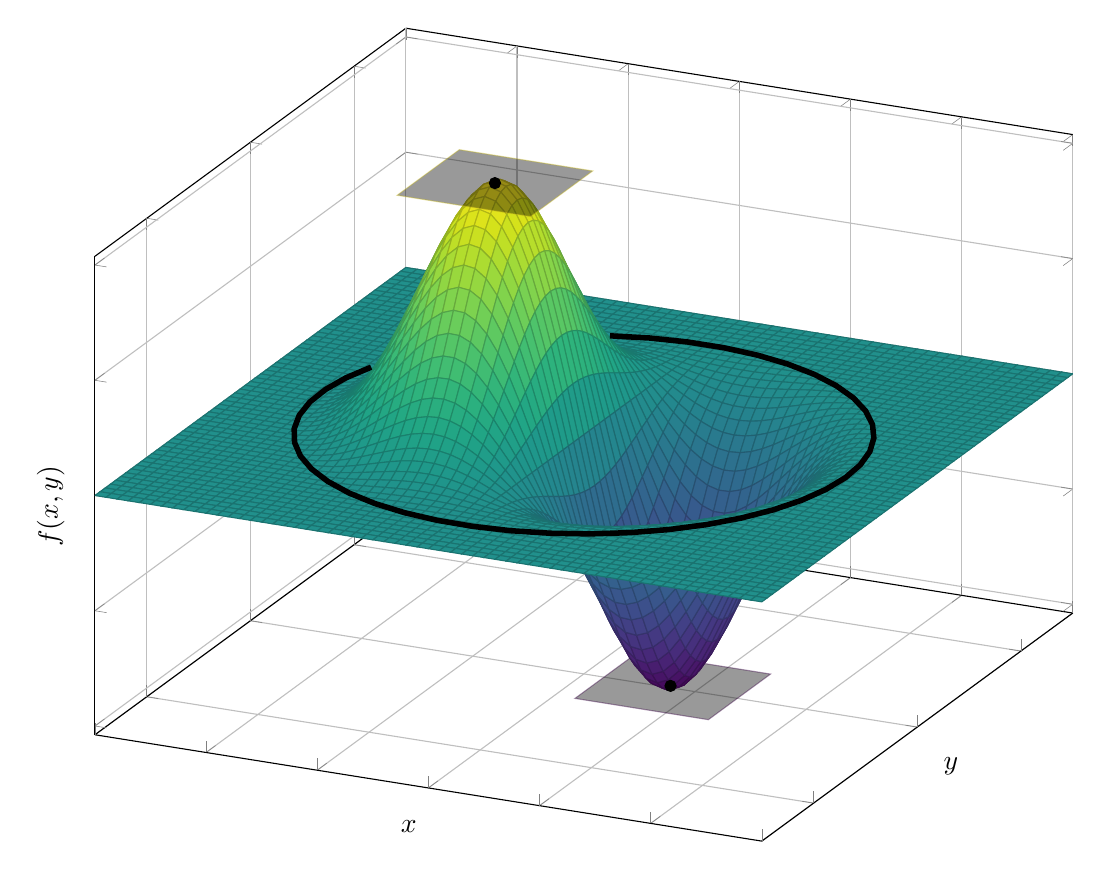
\begin{tikzpicture}
            \begin{axis}[
                colormap name=viridis,
                % 3d box,
                width=14cm,
                view={25}{20},
                axis equal image,
                enlargelimits=false,
                grid=major,
                domain=-1.5:1.5,
                samples=61,
                yticklabels={,,},
                xticklabels={,,},
                zticklabels={,,},
                xlabel=$x$,
                ylabel=$y$,
                zlabel={$f(x, y)$},
                ]
                \addplot3 [y domain = -0.3:0.3, domain = 0.1:0.7, samples=2, surf, opacity=0.4, color=black] {-1.03};
                \addplot3 [y domain = -1.5:1.5, surf]
                    {(1-exp(1.4-x*x-y*y))*x*exp(-x*x-y*y)*max(1.4-x*x-y*y, 0)};
                \addplot3[color=black,
                    samples=40,
                    domain=2.83:8.20,
                    line width=2.0pt,samples y=0]
                ({sqrt(1.4)*cos(deg(x))}, {sqrt(1.4)*sin(deg(x))}, 0);
                \addplot3[mark=*] coordinates {(-0.40,0,1.03)};
                \addplot3[mark=*] coordinates {(0.39,0,-1.03)};
                \addplot3 [y domain = -0.3:0.3, domain = -0.7:-0.1, samples=2, surf, opacity=0.4, color=black] {1.03};
            \end{axis}
    \end{tikzpicture}

\end{document}
